\documentclass[a4paper,14pt]{extarticle}
\usepackage{geometry}
\usepackage[T1]{fontenc}
\usepackage[utf8]{inputenc}
\usepackage[english,russian]{babel}
\usepackage{amsmath}
\usepackage{amsthm}
\usepackage{amssymb}
\usepackage{fancyhdr}
\usepackage{setspace}
\usepackage{graphicx}
\usepackage{colortbl}
\usepackage{tikz}
\usepackage{pgf}
\usepackage{subcaption}
\usepackage{listings}
\usepackage{indentfirst}
\usepackage[
backend=biber,
style=numeric,
maxbibnames=99
]{biblatex}
\addbibresource{refs.bib}
\usepackage[colorlinks,citecolor=blue,linkcolor=blue,bookmarks=false,hypertexnames=true, urlcolor=blue]{hyperref} 
\usepackage{indentfirst}
\usepackage{mathtools}
\usepackage{booktabs}
\usepackage[flushleft]{threeparttable}
\usepackage{tablefootnote}

\usepackage{chngcntr} % нумерация графиков и таблиц по секциям
\counterwithin{table}{section}
\counterwithin{figure}{section}

\graphicspath{{graphics/}}%путь к рисункам

\makeatletter
% \renewcommand{\@biblabel}[1]{#1.} % Заменяем библиографию с квадратных скобок на точку:
\makeatother

\geometry{left=2.5cm}% левое поле
\geometry{right=1.0cm}% правое поле
\geometry{top=2.0cm}% верхнее поле
\geometry{bottom=2.0cm}% нижнее поле
\setlength{\parindent}{1.25cm}
\renewcommand{\baselinestretch}{1.5} % междустрочный интервал


\newcommand{\bibref}[3]{\hyperlink{#1}{#2 (#3)}} % biblabel, authors, year
\addto\captionsrussian{\def\refname{Список литературы (или источников)}} 

\renewcommand{\theenumi}{\arabic{enumi}}% Меняем везде перечисления на цифра.цифра
\renewcommand{\labelenumi}{\arabic{enumi}}% Меняем везде перечисления на цифра.цифра
\renewcommand{\theenumii}{.\arabic{enumii}}% Меняем везде перечисления на цифра.цифра
\renewcommand{\labelenumii}{\arabic{enumi}.\arabic{enumii}.}% Меняем везде перечисления на цифра.цифра
\renewcommand{\theenumiii}{.\arabic{enumiii}}% Меняем везде перечисления на цифра.цифра
\renewcommand{\labelenumiii}{\arabic{enumi}.\arabic{enumii}.\arabic{enumiii}.}% Меняем везде перечисления на цифра.цифра

\begin{document}
\begin{titlepage}
    \begin{center}
        {\footnotesize\bfseries
        ФЕДЕРАЛЬНОЕ ГОСУДАРСТВЕННОЕ АВТОНОМНОЕ ОБРАЗОВАТЕЛЬНОЕ\\
        УЧРЕЖДЕНИЕ ВЫСШЕГО ОБРАЗОВАНИЯ\\
        "НАЦИОНАЛЬНЫЙ ИССЛЕДОВАТЕЛЬСКИЙ УНИВЕРСИТЕТ\\
        "ВЫСШАЯ ШКОЛА ЭКОНОМИКИ"\\
        ФАКУЛЬТЕТ КОМПЬЮТЕРНЫХ НАУК}\\[6em]

        {
        \underline{Кузьмин Дмитрий Андреевич}\\[2em]
        }

        {\bfseries МАГИСТЕРСКАЯ ДИССЕРТАЦИЯ}\\[1em]

        {\bfseries
        \textsc{\underline{Детекция дефектов речи с помощью скороговорок}}\\
        \underline{Detecting speech defects using tongue twisters}
        }\\[3em]

        {по направлению подготовки \underline{01.04.02 Прикладная математика и информатика}\\
        образовательная программа «Искусственный интеллект»
        }\\[6em]
    \end{center}

    \begingroup
    \setlength{\parskip}{0pt}%
    \renewcommand{\baselinestretch}{1}\normalsize
    
    \noindent Студент\\[0.2em]
    \noindent \underline{Д.А. Кузьмин}\\[0.2em]
    
    \begin{flushright}
        Научный руководитель\\[0.2em]
        Доцент ФКН НИУ~ВШЭ\\[0.2em]
        \underline{Е.О. Кантонистова}
    \end{flushright}
    
    \endgroup

    \vfill

    \begin{center}
        {Москва 2026}
    \end{center}
\end{titlepage}% это титульный лист - выберите подходящий вам из имеющихся в проекте вариантов (kr - курсовая работа у 3 курса, vkr - выпускная квалификационная работа у 4 курса)
\newpage
\setcounter{page}{2}

{
	\hypersetup{linkcolor=black}
	\tableofcontents
}

\newpage

\newpage
\section*{Аннотация}
\addcontentsline{toc}{section}{Аннотация}
В данной работе изучается возможность применения методов машинного и глубинного обучения для автоматической детекции дефектов речи у детей по аудиозаписям чтения скороговорок, а также реализован сервис в виде Telegram-бота, задача которого оптимизировать работу преподавателей-логопедов, предоставив возможность быстрой оценки качества детской речи и последующего мониторинга динамики результатов.

Ставится задача бинарной классификации аудиозаписей, в рамках которой изучается зависимость между акустическими характеристиками и наличием нарушений речи.

Для решения задачи используется размеченный датасет из 2776 аудиозаписей, при этом около двух третей записей отнесены к классу «good» (правильное произношение), а остальные — к классу «bad» (произношение с дефектами). В работе сравниваются следующие группы подходов (а также их комбинации): классические методы на основе простых классификаторов и акустических признаках, сверточные и рекуррентные нейронные сети, модели, использующие высокоуровневые эмбеддинги, полученные с помощью предобученных моделей (HuBERT, Whisper, VGGish).

Качество моделей оценивается с помощью метрик accuracy и F1-мера (как общая, в режиме macro, так и по классу «bad», как более значимому). 

Результаты работы показывают, что подходы на основе эмбеддингов предобученных моделей показывают наилучшие метрики. Эти подходы использованы при написании сервиса для логопедической диагностики.

\section*{Ключевые слова}
дефекты речи, скороговорки, аудиоклассификация, предобученные речевые модели, глубинное обучение, MFCC, CNN, RNN, HuBERT, Whisper, VGGish


\section{Введение}

\subsection{Описание предметной области}

Нарушения речи у детей является распространённой проблемой, которая влияет на обучение и социальную адаптацию. В логопедической практике диагностика часто опирается на экспертную оценку произношения, что затратно по времени и затрудняет регулярный мониторинг динамики.

Выделяют широкий спектр нарушений речи как у детей, так и у взрослых, которые имеют разные причины: 
\begin{itemize}
    \item недоразвитость речевого аппарата (возрастная незрелость артикуляционной моторики);
    \item поражение нервной системы (дизартрия, афазия и др.);
    \item дефекты речевого аппарата (ринолалия и др.).
\end{itemize}

В данной работе используются аудиозаписи с нарушениями первого типа. Но, несмотря на различия в причинах, акустические и просодические маркеры схожи при разных типах нарушений речи. Что позволяет использовать результаты исследований, выполненных на ином типе нарушений речи, в качестве источника идей для выбора признаков и архитектур для данной работы.

Скороговорки являются удобным способом для автоматизации оценки, так как это это стандартизированный текст, содержащий речевую нагрузку, которая повышает вероятность проявления артикуляционных ошибок и нарушений речи. Для прикладных систем это важно, поскольку позволяет сравнивать результаты в сопоставимых условиях.

Методы машинного и глубинного обучения делают возможным решение задачи автоматической детекции дефектов речи по аудиозаписям. Системы, построенные с помощью данных методов не могут заменить логопеда, но могут быть инструментом первичного скрининга и мониторинга результатов.

\subsection{Постановка задачи}

В работе решается задача бинарной классификации аудиозаписей детской речи. Для каждой записи чтения скороговорки необходимо предсказать метку класса: «good» (нормальное
произношение) или «bad» (наличие речевого дефекта). Цель --- построить модель, устойчиво работающую на новых записях и пригодную для практического применения.

Формально, пусть $X=\{x_i\}_{i=1}^{N}$ --- множество аудиосигналов, а
$Y=\{y_i\}_{i=1}^{N}$, $y_i \in \{0,1\}$ --- соответствующие метки классов. Требуется построить отображение
\[
f_\theta : \mathcal{X} \rightarrow \{0,1\},
\]
где $\theta$ --- параметры модели, минимизирующие ошибку классификации на отложенной выборке. То есть, мы решаем задачу оценки качества произношения на уровне всей записи.

Дополнительно в работе ставится прикладная цель: определить модель, которая может быть использована в сервисе (Telegram-боте) для помощи логопедам при первичном
скрининге и мониторинге результатов занятий, а также реализация данного сервиса.

\subsection{Анализ датасета}

Для экспериментов используется размеченный датасет из 2776 аудиозаписей чтения
скороговорок детьми. Разметка бинарная: «good» и «bad». Приблизительно две трети записей принадлежат классу «good», что создаёт дисбаланс классов.

Ключевые особенности датасета:
\begin{itemize}
    \item \textbf{Контрольные буквы}: каждое наблюдение (аудиозапись скороговорки) помечено контрольными буквами, это те буквы, нарушение произношения которых проверяет данная скороговорка. Каждое наблюдение помечено хотя бы одной контрольной буквой. Всего контрольных букв 8 (л, р, с, т, ц, ч, ш, щ)
    \item \textbf{Длительность аудиозаписей (сек.)}: минимальная: 0.99, максимальная: 68.66, средняя: 10.36, медианная: 8.84.
    \item \textbf{Ограниченный объём}: 2776 записей недостаточно для обучения крупных моделей с нуля, поэтому особенное внимание уделено методам с использованием предобученных эмбеддингов.
\end{itemize}

Более подробная информация представлена на Рисунке~\ref{fig:dataset}

\begin{figure}[ht]
	\centering
	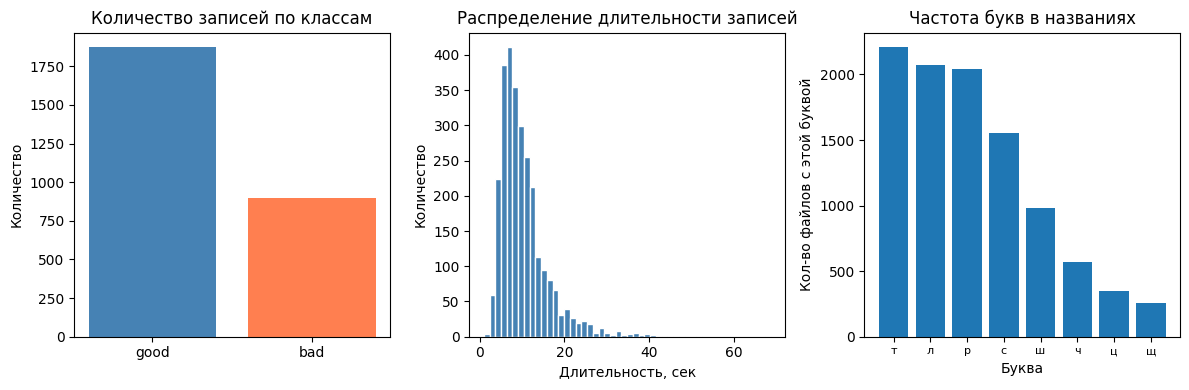
\includegraphics[width=0.95\textwidth]{graphics/dataset.png}
	\caption{Основные параметры датасета}
	\label{fig:dataset}
\end{figure}

Входом моделей является аудиосигнал и производные акустические признаки. Дополнительные признаки наличия контрольных букв используются как вспомогательные там, где это улучшает качество классификации.

\subsection{Выбор метрик и обоснование}

Обозначения (для положительного класса \emph{bad}):
\begin{itemize}
    \setlength{\itemsep}{-5pt}
    \item TP — true positive (верно предсказан класс \emph{bad});
    \item TN — true negative (верно предсказан класс \emph{good});
    \item FP — false positive (предсказан класс \emph{bad}, на самом деле \emph{good});
    \item FN — false negative (предсказан класс \emph{good}, на самом деле \emph{bad}).
\end{itemize}

Метрика $accuracy$ показывает долю правильно классифицированных записей и удобна как общий индикатор работы модели. Однако при дисбалансе классов высокое значение $accuracy$ может достигаться даже при наивном прогнозе самого частого класса. Поэтому $accuracy$ рассматривается как вспомогательная, но не основная метрика.

\[
  \text{Accuracy} = \frac{TP + TN}{TP + TN + FP + FN}
\]

Ключевой метрикой в работе является $F1_{\text{bad}}$, так как именно
класс \emph{bad} соответствует записям с дефектами речи. Эта метрика
объединяет $\text{Precision}_{\text{bad}}$ и $\text{Recall}_{\text{bad}}$, позволяя одновременно контролировать два важных аспекта: не пропускать дефекты и не создавать много ложных срабатываний.

\[
  \text{Precision}_{\text{bad}} =
  \frac{TP}{TP + FP}, \quad
  \text{Recall}_{\text{bad}} =
  \frac{TP}{TP + FN}
\]

\[
  F1_{\text{bad}} =
  2 \cdot
  \frac{\text{Precision}_{\text{bad}} \cdot \text{Recall}_{\text{bad}}}
       {\text{Precision}_{\text{bad}} + \text{Recall}_{\text{bad}}}
\]

Метрика $F1_{\text{macro}}$ усредняется по классам. Для нашей задачи
это особенно важно: модель должна быть одинаково внимательна и к
нормальной речи, и к речи с дефектами. Высокий $F1_{\text{macro}}$
свидетельствует о более сбалансированном поведении модели.

\[
  F1_{\text{macro}} =
  \frac{F1_{\text{good}} + F1_{\text{bad}}}{2}
\]

Таким образом, мы выбираем следующую иерархию важности метрик:
на первом месте — $F1_{\text{bad}}$, на втором — $F1_{\text{macro}}$,
на третьем — $\text{accuracy}$.

\subsection{Результаты работы}

В ходе работы реализованы и сопоставлены результаты нескольких групп моделей: классические ML-подходы на акустических признаках, нейросетевые модели на спектральных представлениях, а также решения на предобученных речевых эмбеддингах. Оценка качества проводилась по метрикам $F1_{bad}$, $F1_{macro}$ и $accuracy$.

Полученные результаты показывают, что на рассматриваемом датасете наилучшее качество демонстрируют подходы на предобученных представлениях. В частности, лидерами стали модели на основе HuBERT и Whisper. 

По итогам экспериментов сформирована основа для внедрения модели в прикладной сервис (Telegram-бот), ориентированный на первичный скрининг и мониторинг динамики качества речи.


\section{Обзор литературы}

\subsection{Классические ML-модели, общие подходы}

Авторы статьи \textbf{\cite{methods_defective_speech_rus}} дают общий обзор подходов к распознаванию дефектной речи и показывают, как  последовательно решаются задачи выделения признаков, нормализации и классификации.

Работа \textbf{\cite{su2018_acoustic_predictors_pediatric_dysarthria}} показывает методы выделения акустических признаков из аудиозаписей речи детей с дизартрией при ДЦП (детский церебральный паралич). Затем авторы применяют отбор признаков и логистическую модель, показывая, какими именно параметрами отличается патологическая речь от нормы.

В работе \textbf{\cite{ng2022_child_ssd_posterior}} авторы построили модель бинарной классификации нарушения звукопроизношения (Speech Sound Disorders, SSD) на базе мел-частотных кепстральных коэффициентов (mel-frequency cepstral coefficients, MFCC). В качестве классификатора в данной работе используется метод опорных векторов (Support Vector Machine, SVM). Модель обучалась на датасете аудиозаписей дошкольников на китайском языке. Статья показывает, что даже без тяжелых моделей можно стабильно решать задачу бинарной классификации дефектов речи.

Статья \textbf{\cite{khomenko2024_diag_doshkolniki}} исследует общую проблему дефектов речи у дошкольников. Помимо логопедической и педиатрической методологии в работе присутствует статистика дефектов речи по звукам, что может быть полезно.

\subsection{DL-модели}

В работе \textbf{\cite{hershey2017_cnn_audio}} на датасете YouTube-100M последовательно сравниваются разные сверточные нейронные сети (convolutional neural network, CNN) такие как AlexNet, VGG, Inception V3, ResNet-50 для решения задачи классификации. Несмотря на то, что в работе решается задача классификации аудио на классы: речь, пение, звуки машины, и т.д., для задачи классификации дефектов речи статья важна как архитектурная база.

Авторы статьи \textbf{\cite{kuo2022_chinese_ssd}} обучают несколько CNN (EfficientNet, DenseNet, \\ Inception V3) на лог-мел спектрограммах детской китайской речи с метками наличия нарушений речи и показывают, что сеть сама извлекает устойчивые временно-частотные паттерны нарушений.

В работе \textbf{\cite{voice_disorders_deeplearning_2025}} рассматриваются аудиозаписи пациентов с различными типами нарушений голосовых связок (повреждение, паралич, одностороннее нарушение) и строится ResNet18 классификатор по мел-спектрограммам. Авторы также сравнивают бинарную и мультиклассовую постановки задачи.

Для детекции заиканий авторами статьи \textbf{\cite{kourkounakis2021_fluentnet}} предлагается архитектура FluentNet, объединяющая ResNet, BiLSTM и attention-блок. Статья показывает, что комбинация локальных признаков и долгосрочной временной динамики позволяет лучше выделять паттерны заикания.

В исследовании \textbf{\cite{kaushik2021_slinet}} для детекции детских дефектов речи предлагается архитектура нейронной сети SLINet по спектрально-временным признакам. Авторы ставят задачу на использование своей модели на небольших устройствах, поэтому особое внимание уделено скорости инференса.

Статья \textbf{\cite{liu2021_swin_transformer}} описывает иерархический Swin Transformer со скользящими окнами и показывает, как организовать масштабируемую attention-обработку с линейной сложностью по размеру входа. Хотя работа из области CV (computer vision, компьютерное зрение), её методы позволят строить более сильные модели аудиоклассификации за счёт многоуровневого извлечения признаков из спектрограмм речи.

Авторы статьи \textbf{\cite{kim2024_ssd_age_bias}} решают проблему детекции нарушений речи на датасете детских аудиозаписей на корейском языке. Особенность подхода, описанного в данной статье в том, что помимо выделения признаков с помощью CNN, используется multi-head архитектура, в которой каждой выходной "голове" соответствует своя возрастная группа (например, 2–4, 5–7, 8–10 лет), что помогает модели фокусироваться на дефектах речи, свойственных для определенного возраста.

\subsection{Модели, использующие высокоуровневые эмбеддинги}

В статье \textbf{\cite{baevski2020_wav2vec2}} представлена модель wav2vec 2.0. В контексте нашей работы можно использовать wav2vec 2.0, обученный на большом корпусе неразмеченной речи, как источник эмбеддингов.

Аналогично предыдущему источнику, статья \textbf{\cite{hsu2021_hubert}} описывает HuBERT, эмбеддинги которого содержат информацию как о фонетике, так и о более высокоуровневых шаблонах и также могут быть использованы в задаче детекции дефектов речи. 

Очередная статья \textbf{\cite{cramer2019_openl3}} описывает L3-Net сеть, предобученную реализацию которой (например OpenL3) можно использовать для получения высокоуровневых эмбеддингов.

Авторы \textbf{\cite{qi2021_fhvae_disorder}} применяют расширенный FHVAE (Factorized Hierarchical \\ Variational Autoencoder, Факторизованный иерархический вариационный автокодировщик), где латентное пространство разделяется на z1 и z2 компоненты (кратковременные и долговременные), а затем объединяются для классификации типов речевых нарушений. Таким подходом авторы пытаются разделить латентные признаки, отвечающие за нарушения речи от признаков, соответствующих конкретному диктору. В работе классифицировалась взрослая речь с патологиями.

В статье \textbf{\cite{jain2023_whisper_child_speech}} исследуется адаптация Whisper к детской речи. Авторы показывают, что дообучение Whisper на датасете детских аудиозаписей повышает точность ASR (Automatic Speech Recognition, автоматическое распознавание речи).

Авторы статьи \textbf{\cite{usefulness_asr_ssd_2025}} используют предобученную модель wav2vec2‑XLS‑R‑1B, дообучив ее на небольшом датасете (1,5 часа) детской речи с дефектами на корейском языке. Авторы показывают, что после дообучения модель не только лучше распознает детскую речь, но и предоставляет эмбеддинги, которые содержат информацию о дефектах речи и помогают в классификации.

В данной работе \textbf{\cite{asr_screening_children_2024}} сравниваются несколько эмбеддинг подходов (wav2vec2, Whisper, Conformer) для решения задачи ASR детской речи.

В работе \textbf{\cite{huang2024_hybrid_module_transformer}} предлагается гибридная модель HuBERT+LSTM+ResNet с модулем слияния признаков, для решения задачи определения эмоций по аудиозаписи. Статья показывает, что комбинирование разных уровней эмбеддингов речи даёт более надёжную классификацию.

Авторы \textbf{\cite{raghu2025_multilingual_dysarthria}} описывают модель, в которой одновременно решается несколько задач: детекция дизартрии, оценка тяжести и ASR. В работе показано, что единое эмбеддинг-пространство может выполнять сразу несколько задач, повышая степень практической применимости модели.

\subsection{Выводы из обзора литературы}

Проведенный анализ литературы показывает, что для задачи автоматической детекции дефектов речи у детей наиболее перспективно проводить эксперименты со следующими подходами (или их комбинациями): классические интерпретируемые признаки, DL-архитектуры на спектрограммах и модели на высокоуровневых эмбеддингах. На основе этого в работе планируется следующая серия экспериментов.

\textbf{1. Эксперименты с классическими ML-моделями на акустических признаках.}
Планируется построить baseline-модели (SVM, Random Forest, Logistic Regression) на признаках MFCC, просодики и vocal-tract характеристиках, чтобы получить интерпретируемую отправную
точку и оценить вклад отдельных акустических индикаторов в качество классификации. Этот блок опирается на подходы и выводы работ~\cite{methods_defective_speech_rus,su2018_acoustic_predictors_pediatric_dysarthria,ng2022_child_ssd_posterior}.

\textbf{2. Эксперименты со спектральными DL-моделями.}
Планируется сравнить 2D CNN, CNN+RNN/attention и transformer-подходы на спектральных представлениях, чтобы проверить, какие архитектуры лучше улавливают паттерны дефектной речи. Данный блок опирается на статьи
\cite{hershey2017_cnn_audio,kuo2022_chinese_ssd,voice_disorders_deeplearning_2025,kourkounakis2021_fluentnet,kaushik2021_slinet,liu2021_swin_transformer,kim2024_ssd_age_bias}.

\textbf{3. Эксперименты с высокоуровневыми эмбеддингами.}
Планируется использовать готовые и дообученные эмбеддинги wav2vec2, HuBERT, Whisper, OpenL3, а также гибридные схемы (например, HuBERT+LSTM+ResNet), чтобы оценить переносимость предобученных представлений на небольшой датасет скороговорок и устойчивость к вариативности
детской речи. Этот блок опирается на работы
\cite{baevski2020_wav2vec2,hsu2021_hubert,cramer2019_openl3,qi2021_fhvae_disorder,jain2023_whisper_child_speech,usefulness_asr_ssd_2025,asr_screening_children_2024,huang2024_hybrid_module_transformer,raghu2025_multilingual_dysarthria}.

\textbf{4. Единая схема оценки и итоговое сравнение.}
Во всех группах моделей планируется использовать единый протокол оценки по метрикам accuracy, F1-macro, F1-bad и времени обучения.
Итогом станет выбор архитектуры, обеспечивающей лучшее качество.
	
\newpage 
\printbibliography[heading=bibintoc] 

\newpage
\appendix

\end{document}
